\section{Problem Formulation}


Recent literature shows that model-based, model-free and hybrid control strategies have been used to control soft robots. However, the developed model-based control algorithms predominantly used kinematic descriptions of the robot rather than dynamical models. Although there are studies that use dynamical models  \cite{falkenhahn2016dynamic}, \cite{della2020model}, and \cite{kapadia2011task}, the field of model-based control applied to soft robots is still under-developed as of today. In this work we aim to find an model-based control strategy that will generally result in higher tracking performance of the soft robot. Hence, the research questions follows:



\textit{Can we develop a model-based control strategy for a pneumatically actuated, 2-link planar soft robot to perform a reference tracking problem?}




\begin{figure}[H]
    \centering
    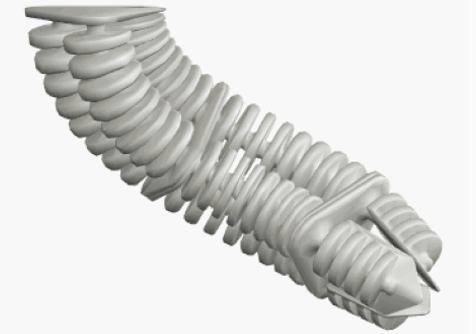
\includegraphics[width = 0.6\textwidth]{Figures/sorotoki1.png}
    \caption{Computer image of a soft robot, the robot we will be using will be of a planar type.}
    \label{fig:sorotoki}
\end{figure}


\section{Approach}

In order to effectively answer the research question several steps need to be taken, a brief description of these steps will be given. First, the dynamic model that has been developed by \cite{caasenbrood2020}, will have to be validated. This validation will be done with the robotic manipulator as was used in \cite{berkers}. This is a planar robot with roughly two degrees of freedom, as it can extend and rotate in plane, and two inputs.

First, the stiffness matrix used in the model will be approximated by a FEM analysis. By applying pressure to a FEM model of the planar robot, a relation between pressure and deformation can be obtained at equilibrium state. After this, the model validation will involve a controlled inflation/deflation of the bellows. In this way the actual elongation and rotation of the soft robot can be compared to the model. This experiment will also be used as a parameter identification, to determine for instance permeability. In order to carry out this first experiment, a simple controller needs to be designed to bring the bellows to a certain pressure. This can be thought of as simple PD controller, where the work of \cite{proper} can be used.

Once the dynamic model has been validated and, if necessary, adapted, a first try will be made to develop a model-based controller. To this end, theory presented in \cite{della2019exact} and \cite{spong1996energy} will have to be applied. The goal will be to carry out a reference tracking problem with this single link robot.  

Once a model-based controller has been established for this 1-link planar soft robot, an additional link will be added to the first link. This will further increase the dexterity of the robot, and will cause non-uniqueness of some end-effector positions. Therefore, a redesign of the model-based controller will be necessary. Once this controller has been developed our goal is to carry out reference tracking problem. 

When the controller provides satisfactory results, a gripper will be mounted to the second link, enabling it to grasp objects. With the addition of the gripper, extra mass is added to the system which is not accounted for in the current dynamic model. Experiments will need to be conducted to see if the dynamic model will have to be revised. Once the gripper is accounted for in the dynamic model, a final reference tracking problem can be executed.

During this project, we aim to develop a new way of sensing as this is a common obstacle in soft robotics. The current set-up allows us to measure rotation of the end-effector with an Inertial Measurement Unit (IMU), and measure translation with a vision system. In order to improve rotation and position data, we want to incorporate sensor fusing. This means that data from the vision system is combined with IMU output to enhance rotation measurement. In practice this can be thought of as two LED's positioned near the end-effector. Based on the measured position data of each LED, a rotation of the end-effector can be determined. This information is then combined with the IMU output to improve rotation measurement. Also, the use of two LED's improve the translation measurement, as an average can be calculated based on the two measured LED positions.
\newpage
Although a 3-bellow soft-robot is present, this research will only focus on developing a model-based controller for the 2-link planar soft robot. Limited laboratory access, resulting in limited experimentation time is the main reason for this. The set-up that is currently present at the laboratory enables us to develop a model-based controller without many changes to the set-up. In this way, valuable research on model-based control of soft-robotics can still done, while respecting the amount of experimentation time available.



%Starting with this less complex planar robot will make it easier to understand and adapt the dynamic model, additionally one will get affinity with the set-up. Once, the dynamic model has been validated and, if necessary, adapted, the planar robot will be replaced by a 1-link robot. This robot has three bellows, which increases the dexterity and degrees of freedom of the robot. With this 1-link robot the earlier determined parameters might have changed, so a parameter identification is necessary at first. After that, a first try will be made to develop a model-based controller. To this end, theory presented in \cite{della2019exact} and \cite{spong1996energy} will have to be applied. The goal will be to carry out a reference tracking problem with this single link robot.  

%Once a model-based controller has been established for the 1-link soft robot, an additional link will added to the first link. This will further increase the dexterity of the robot, and will cause non-uniqueness of some end-effector positions. Therefore, a redesign of the model-based controller will be necessary. Once this controller has been developed our goal is to carry out reference tracking problem.

%When the controller provides satisfactory results, a gripper will be mounted to the second link, enabling it to grasp objects. With the addition of the gripper, extra mass is added to the system which is not accounted for in the current dynamic model. Experiments will need to be conducted to see if the dynamic model will have to be revised. Once the gripper is accounted for in the dynamic model, a final reference tracking problem can be executed.
